\chapter[Przegląd czujników ultradźwiękowych]{Przegląd czujników ultradźwiękowych}

\label{chapter:przeglad_czujnikow}
Jedną z najważniejszych części projektu jest układ odbiorczy. 
Wybrane elementy muszą spełniać szereg założeń niezbędnych do poprawnego zrealizowania zadania. 
W tym rozdziale przedstawiony jest proces doboru elementów składających się na finalny odbiornik.



% Proszę opisać kilka wybranych, możliwie reprezentatywnych
% dalmierzy ultradźwiękowych.

\section{Dobór odbiornika}
Wymagania jakie powinien spełniać odbiornik wynikają bezpośrednio z założeń projektu. 
Pierwszym z nich jest czułość przetwornika na częstotliwości ultradźwiękowe. Na rysunku \ref{fig:mic_response} 
widzimy przykładowy wykres pasma przenoszenia mikrofonu w odniesieniu do częstotliwości \unit[1]{kHz}. 
W przypadku docelowego czujnika istotna jest czułość w wąskim paśmie \unit[40]{kHz}. 
Czułość ta nie powinna znacząco odbiegać poniżej czułości referencyjnej, a w tym przypadku wynosi \unit[-2]{dB}, co jest akceptowalną wartością.
Dokładna częstotliwość podyktowana jest głównie standardami branży. Większość przetworników piezoelektrycznych, 
służących do generowania sygnału ma swój punkt rezonansu w wąskim paśmie bliskim \unit[40]{kHz}.

\begin{figure}[ht!]
    \centering
    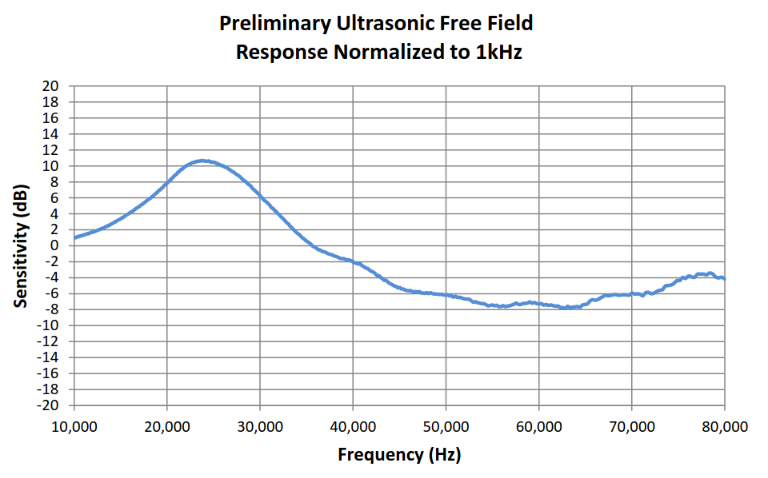
\includegraphics[width=0.8\textwidth]{mic_response.png}
    \captionsource{Pasmo przenoszenia mikrofonu SPU0410LR5H-QB}{\cite{knowles:SPU0410LR5H}}
    \label{fig:mic_response}
\end{figure}

\noindent

Następnym wymaganiem jest rozmiar. 
Wynika to z rodzaju wykonywanego pomiaru. Każdy z czujników wykrywa przejście sygnału przez poziom wartości zerowej. 
Odbiorniki nie powinny być oddalone od siebie bardziej niż połowa długości fali dźwiękowej. 
To zapewnia, że pomiary będą dotyczyły tego samego czoła fali. W przeciwnym przypadku zrealizowane pomiary nie pozwalałyby jednoznacznie wyznaczyć kąta jej padania.
Długość fali jest zależna od częstotliwości sygnału oraz jego prędkości rozchodzenia się w danym medium. 
Wyznaczamy ją ze wzoru \ref{eq:wavelength}, przy czym częstotliwość jest równa \unit[40]{kHz},
a {\em prędkość rozchodzenia się dźwięku w powietrzu przy temperaturze 15 °C wynosi \unit[340,3]{m/s}} \cite{sound_speed}.
Połowa długości fali to zatem \unit[4,25]{mm} i tej wartości nie powinna przekraczać odległość między odbiornikami.
Wszystkie czujniki tak małych rozmiarów są produkowane w technologii MEMS. 
\begin{equation}
\lambda = \frac{v}{f} = \frac{340,3\frac{m}{s}}{40kHz}=0,0085m = 8,5mm
\label{eq:wavelength}    
\end{equation}

\noindent
\vspace{2cm}

Kolejnym wymaganiem jest takie umieszczenie otworu ciśnieniowego w obudowie, by był skierowany on wewnątrz laminatu obwodu drukowanego. 
Taka konstrukcja, jak na rysunku \ref{fig:mic}, pozwala na stworzenie płaskiej powierzchni, tylko z otworami ciśnieniowymi czujników. 
Przekłada się to na mniejsze zakłócenia spowodowane odbiciami fali dźwiękowej od elementów elektronicznych.

\begin{figure}[ht!]
    \centering
    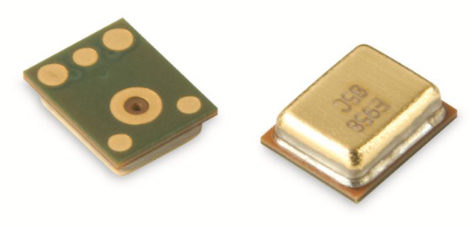
\includegraphics[width=0.8\textwidth]{mic.png}
    \captionsource{Mikrofon SPU0410LR5H-QB}{\cite{knowles:SPU0410LR5H}}
    \label{fig:mic}
\end{figure}
\noindent
Ostatecznym wymaganiem była dostępność i przystępność cenowa produktu. Ze względu na tak rygorystyczne oczekiwania wybór zawęził się zaledwie do kilku pozycji.
Jedną z nich był mikrofon SPU0410LR5H-QB marki Knowles\cite{knowles}, który w odpowiedniej liczbie został dostarczony przez Promotora.
\vspace{2cm}



\section{Komercyjne rozwiązania}
Rynek obfituje w rozwiązania z wykorzystaniem ultradźwiękowych czujników odległości, 
ale względnie niewiele firm oferuje sonary bez ruchomych elementów.
Czołowym producentem urządzeń w takiej technologii jest TOPOSENS ze swoim produktem o nazwie ECHO ONE\textregistered.
Rysunek \ref{fig:echoone}, który jest zdjęciem marketingowym produktu, sugeruje, 
że posiada on ultradźwiękowy nadajnik oraz trzy odbiorniki we wzorze tworzącym kąt prosty.

\begin{figure}[ht!]
    \centering
    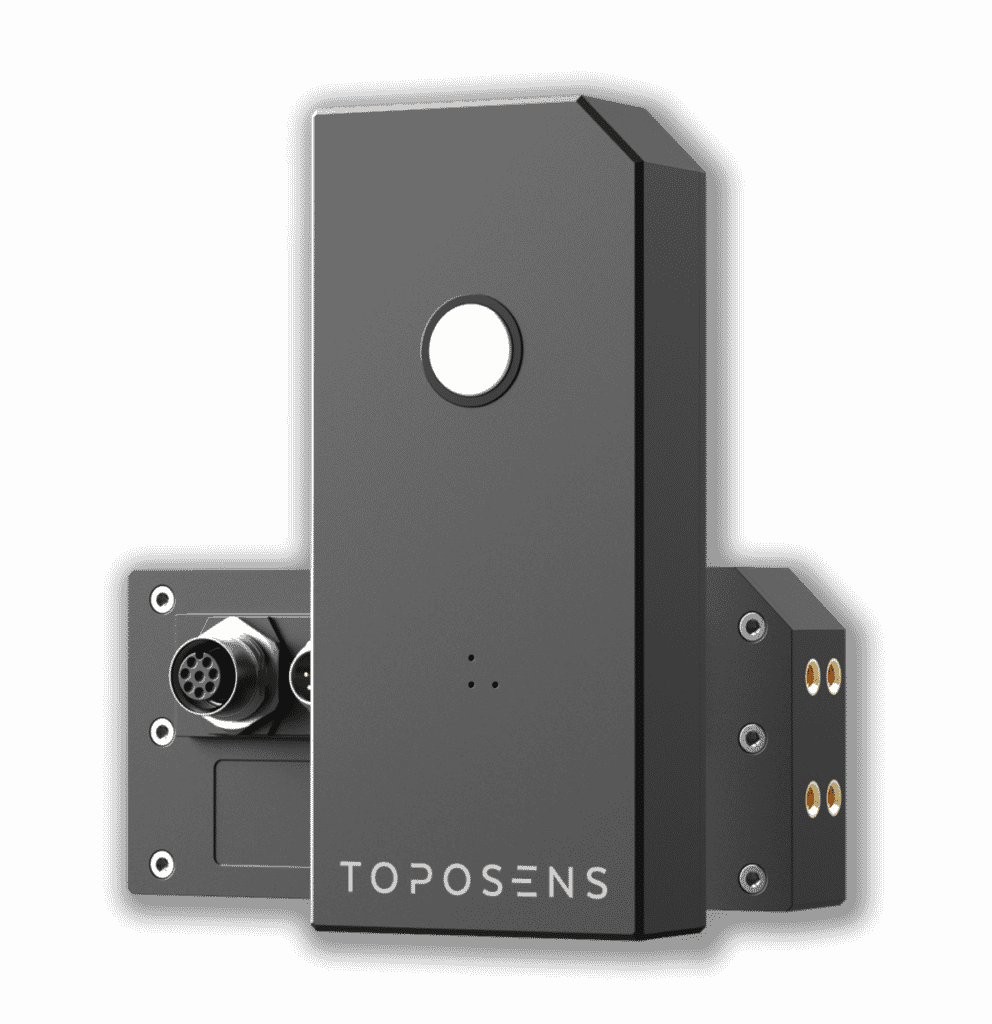
\includegraphics[width=0.5\textwidth]{ECHOONE.png}
    \captionsource{TOPOSENS ECHO ONE}{\url{https://toposens.com/}}
    \label{fig:echoone}
\end{figure}
